\section{Étude de coûts}

\begin{figure}[h]
        \centering
        \begin{subfigure}[t]{0.4\textwidth}
            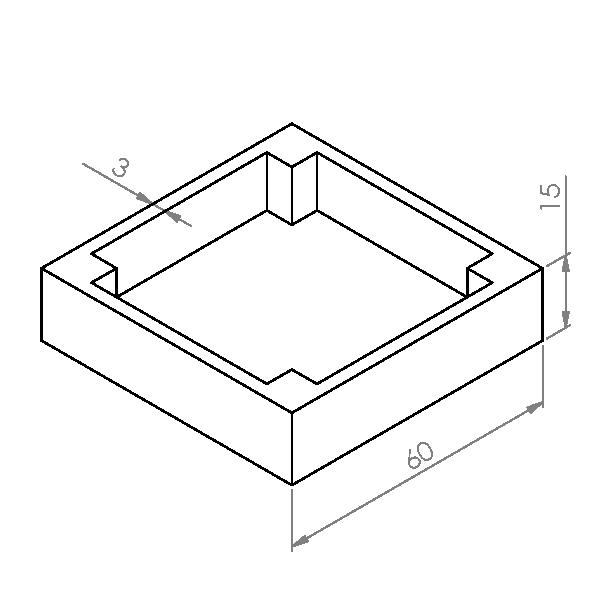
\includegraphics[width=\textwidth]{images/example_part/example_mid}
            \caption{Partie mécanique. Dimensions en \si{\milli\meter}.}
        \end{subfigure}
        ~
        \begin{subfigure}[t]{0.4\textwidth}
                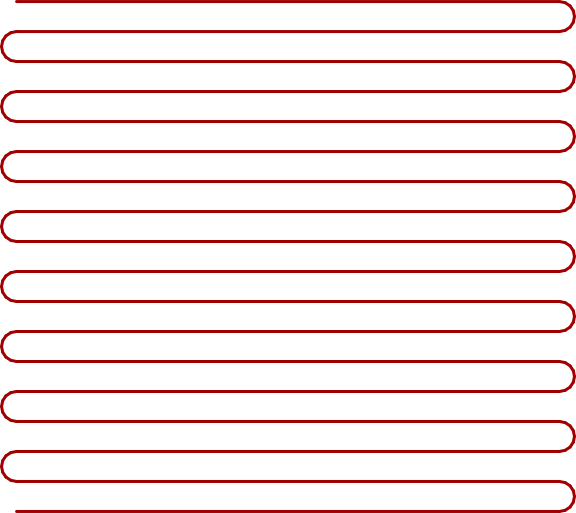
\includegraphics[width=\textwidth]{images/example_part/tracks.png}
                \caption{Tracé des pistes (similaire pour les cinq faces intérieures).}
        \end{subfigure}

        \caption{Pièce d'exemple. Les dimensions et la géométrie sont approximatives. La largeur des pistes et la distance entre deux pistes est de \SI{150}{\micro\meter}.}
        \label{fig:example-part}
\end{figure}
Pour notre étude de coûts, nous avons décidé de nous baser sur la série en production chez Cicorel lors de notre visite.
Les tableaux de calculs de coûts restent néanmoins généralisables, moyennant un changement de certaines valeurs.
Les paramètres à changer en fonction de la pièce sont indiqués dans le détail de chaque partie.


\paragraph{Descriptif de la pièce}
La pièce que nous considérons est une pièce relativement simple.
Il s'agit d'un couvercle contre l'ingénierie inverse pour lecteur de carte de crédit.
Le rôle de cette pièce est de détecter toute tentative d'accéder à l'intérieur de l'appareil, soit en le démontant, soit en le perçant.
Pour accomplir cette fonction, deux pistes sont placées en serpentin à l'intérieur du couvercle.
L'appareil est programmé pour effacer toute les données sensibles dès qu'une de ces pistes est rompue.
Cette pièce était malheureusement confidentielle et nous n'avons pas pu la prendre en photo.
On peut l'approximer par la boîte creuse visible à la fig. \ref{fig:example-part}.


\subsection{Injection}
\begin{table}[h!]
\centering 
\begin{tabular}{l S[table-format=3.2] r} 
\toprule 
\multicolumn{2}{l}{\textbf{Électricité}} & \\ 
Consommation électrique & 5 & \si{\kilo\watt} \\
Prix de l'électricité & 0.2 & \si{\chf\per\kilo\watt\per\hour} \\
\cmidrule(l){2-3}
Coût d'électricité & 1 & \si{\chf\per\hour} \\
\midrule
\multicolumn{2}{l}{\textbf{Machines}} & \\ 
Presse électrique & 130000 & \si{\chf} \\
Fonctionnement & 6240 & \si{\hour\per\annee} \\
\cmidrule(l){2-3}
Amortissement sur 5 ans & 4.17 & \si{\chf\per\hour} \\
\midrule
\multicolumn{2}{l}{\textbf{Opérateurs}} & \\ 
Opérateur à 10\% & 6& \si{\chf\per\hour} \\
\midrule

\multicolumn{2}{l}{\textbf{Matière}} & \\ 
Matière (\textsc{pc}) & 11 & \si{\chf\per\kilogram} \\ 
Poids de la pièce & 25 & \si{\gram} \\
\cmidrule(l){2-3}
Coût de la matière & 0.27 & \si{\chf\per\piece} \\

\midrule
\multicolumn{2}{l}{\textbf{Outillage}} & \\ 
Prix du moule & 20000 & \si{\chf} \\
Pièces par série & 20000& \si{\piece} \\
\cmidrule(l){2-3}
Coûts d'outillage & 1 & \si{\chf\per\piece} \\

\midrule
\midrule
Coût horaire & 11.67  & \si{\chf\per\hour} \\
Temps de cycle & 20 & \si{\second\per\piece} \\
\cmidrule(l){2-3}
\textbf{\textsc{Total}} & 1.34 & \si{\chf\per\piece} \\

\bottomrule 
\end{tabular}
\caption{Calcul des coûts de l'injection plastique} 
\label{tab:cost-molding}
\end{table}



L'étape d'injection plastique demande un moule usiné soit par éléctroérosion, soit par usinage à grande vitesse.
Le coût du moule a été estimé suivant les calculs présentés dans le séminaire\cite{electroerosion-2013}.
Le détail de ces calculs sortant du cadre du présent séminaire, nous avons fait le choix de ne pas les inclure. 

Nous avons également supposé que la pièce est réalisée dans la matière la moins chère, c'est à dire le polycarbonate.
Les polymères activables sont en moyenne 20\% plus cher que leur homologue non activable d'après notre contact chez Cicorel.
Les prix des matériaux varient entre \SI{11}{\chf\per\kilogram} pour du \textsc{pc} et \SI{220}{\chf\per\kilogram} pour du \textsc{peek}.
\clearpage

\subsection{Activation Laser}
Pour calculer le coût de l'étape d'activation sélective (\gls{lds}) nous avons fait quelques hypothèses :
\begin{itemize}
    \item Le secteur d'activation laser tourne \SI{24}{\hour} par jour, 5 jours sur 7.
    \item La machine est une Microline 160i de chez LPKF coûtant \SI{220000}{\chf}.
        Elle est amortie en 5 ans.
    \item Un opérateur ne peut s'occuper que d'une machine à la fois.
    \item La machine consomme en permanence sa puissance de pointe soit \SI{2.5}{\kilo\watt} \cite{lpkf-microline-series}.
        L'électricité représentant une fraction faible du coût final, cette hypothèse n'induit pas de grandes erreurs.
\end{itemize}

Le calcul de la surface occuppée par les pistes sur notre circuit se base sur une largeur de piste de \SI{150}{\micro\meter} et une
distance entre deux pistes de \SI{150}{\micro\meter} également, pour une piste occupant toute la surface du circuit.
Pour une autre pièce, la surface des pistes peut souvent être obtenue dans le logiciel de conception.

\begin{table}[h!]
\centering 
\begin{tabular}{l S[table-format=3.2] r} 
\toprule 
\multicolumn{2}{l}{\textbf{Électricité}} & \\ 
Consommation électrique & 2.5 & \si{\kilo\watt} \\
Prix de l'électricité & 0.2 & \si{\chf\per\kilo\watt\per\hour} \\
\cmidrule(l){2-3}
Prix de l'électricité & 0.5 & \si{\chf\per\hour} \\
\midrule
\multicolumn{2}{l}{\textbf{Machines}} & \\ 
LPKF Microline 160i & 220000 & \si{\chf} \\
Fonctionnement & 6240 & \si{\hour\per\annee} \\
\cmidrule(l){2-3}
Amortissement sur 5 ans& 7.05 & \si{\chf\per\hour} \\
\midrule
\multicolumn{2}{l}{\textbf{Opérateurs}} & \\ 
Opérateur à 100\% & 60& \si{\chf\per\hour} \\

\midrule
\multicolumn{2}{l}{\textbf{Temps de cycle}} & \\ 
Vitesse du laser & 4000 & \si{\milli\meter\per\second} \\
Diamètre du laser & 80 & \si{\micro\meter} \\
Vitesse de balayage & 320 & \si{\milli\meter\squared\per\second} \\
Surface des pistes & 1800 & \si{\milli\meter\squared\per\piece} \\ 
Temps de balayage & 5.625 & \si{\second\per\piece} \\ 
Temps de positionnement & 1 & \si{\second\per orientation} \\
Nombre d'orientations & 5 &  \\
Temps de mise en place, retrait et inspection & 15 & \si{\second\per\piece} \\ 

\cmidrule(l){2-3}
\textbf{Temps total} & 25.625 & \si{\second\per\piece} \\ 

\midrule
\midrule
Coût horaire & 67.68 & \si{\chf\per\hour} \\
Temps de cycle & 25.625 & \si{\second\per\piece} \\
\cmidrule(l){2-3}
\textbf{\textsc{Total}} & 0.48 & \si{\chf\per\piece} \\

\bottomrule 
\end{tabular}
\caption{Calcul des coûts de l'activation sélective par laser} 
\label{tab:cost-laser-activation}
\end{table}


\subsection{Métallisation}
Calculer le coût réel de cette étape est difficile, car beaucoup d'informations ne sont pas accessibles publiquement : le prix des bains et de la \gls{step} pour ne citer que ces deux là, ne sont pas disponibles chez les fournisseurs.
De plus, filtrer les bains pour les recycler permet de récupérer un peu de matière qui est revendue, ce qui intervient dans le calcul de coût, mais est difficile à estimer.
Finalement, notre contact chez Cicorel a refusé de détailler leur méthode de calculs pour ces bains, en nous répondant qu'il s'agissait de données internes et confidentielles.

Nous avons donc estimé que le coût pour déposer \SI{1}{\kilogram} de métal par voie chimique était environ cinq fois le prix de ce métal sur le marché.
Ce coût inclut la \gls{step}, le chauffage des bains et l'électricité consommée par le robot servant à déplacer les pièces d'un bain au suivant. 
Cette estimation peut sembler hasardeuse, mais elle donne néanmoins une approximation suffisante pour l'ingénieur désireux d'utiliser ce procédé.
À ce coût, il faut ajouter l'amortissement de la machine sur cinq ans et l'opérateur (deux opérateur pour trois lignes).

Pour estimer le temps de cycle, nous avons retenu le temps de l'étape la plus longue, c'est à dire la déposition du cuivre.
En effet, une fois un rack sorti du bain de cuivre, un autre peut prendre sa place tandis que le premier continue dans la chaîne.

\begin{table}[h!]
\centering 
\begin{tabular}{l S[table-format=3.2] r} 
\toprule 
\multicolumn{2}{l}{\textbf{Machines}} & \\ 
Chaîne de bains& 1000000 & \si{\chf} \\
Fonctionnement & 6240 & \si{\hour\per\annee} \\
\cmidrule(l){2-3}
Amortissement sur 5 ans & 32& \si{\chf\per\hour} \\
\midrule
\multicolumn{2}{l}{\textbf{Opérateurs}} & \\ 
Opérateur à 66\% & 40& \si{\chf\per\hour} \\
\midrule

\multicolumn{2}{l}{\textbf{Matière}} & \\ 
Cuivre chimique & 100 & \si{\chf\per\kilogram} \\ 
Nickel chimique & 100 & \si{\chf\per\kilogram} \\ 
Or chimique & 175000 & \si{\chf\per\kilogram} \\ 
Couche de cuivre (\SI{6}{\micro\meter}) & 5.34 & \si{\chf\per\meter\squared} \\
Couche de nickel (\SI{6}{\micro\meter}) & 5.34 & \si{\chf\per\meter\squared} \\
Couche d'or (\SI{0.05}{\micro\meter}) & 168.875 & \si{\chf\per\meter\squared} \\
Surface de piste & \num{3e-3} & \si{\meter\squared\per\piece} \\ 
\cmidrule(l){2-3}
Coût de la matière & 0.54 & \si{\chf\per\piece} \\

\midrule
\midrule
Coût horaire & 72 & \si{\chf\per\hour} \\
Temps de cycle & 2 & \si{\hour} \\
Pièces par bain & 400 & \\
\cmidrule(l){2-3}
\textbf{\textsc{Total}} & 0.90 & \si{\chf\per\piece} \\

\bottomrule 
\end{tabular}
\caption{Calcul des coûts de la métallisation.} 
\label{tab:cost-metallization}
\end{table}


\clearpage % TODO changer ca !
\subsection{Récapitulatif}
Le calcul des coût appliqué au couvercle d'exemple (fig. \ref{fig:example-part}) donne le résultat visible dans le tab. \ref{tab:cost-final}.
Les fig. \ref{fig:cost-repartition} et \ref{fig:cost-repartition-b} montrent la répartition des coûts en fonction de l'étape de fabrication et de leur source.
\begin{table}[h!]
\centering 
\begin{tabular}{l S[table-format=3.2] r} 
\toprule 
Injection & 1.34 & \si{\chf\per\piece} \\
Activation sélective & 0.47 & \si{\chf\per\piece} \\  
Métallisation & 0.70 & \si{\chf\per\piece} \\ 
\cmidrule(l){2-3}
\textbf{\textsc{Total}} & 2.51 & \si{\chf\per\piece} \\

\bottomrule 
\end{tabular}
\caption{Récapitulatif des coûts.} 
\label{tab:cost-final}
\end{table}





\begin{figure}[p!]
    \begin{tikzpicture}
        \pie[sum=auto,text=pin, explode=0.1, after number=\si{\chf}, color=lightgray]{0.38/Injection, 0.55/LDS, 0.90/Métallisation}
    \end{tikzpicture}
    \begin{center}
        \caption{Répartition des coûts selon les étapes pour la pièce d'exemple.}\label{fig:cost-repartition}
    \end{center}
\end{figure}

\begin{figure}[p!]
    \begin{tikzpicture}
        \pie[sum=auto,text=pin, explode=0.1, color=lightgray]{72/Opérateur, 24/Amortissement, 54/Bains, 4/Moule,27.5/Matière}
    \end{tikzpicture}
    \begin{center}
        \caption{Source des différents coûts (en centimes). L'électricité n'est pas affichée, car négligeable.}
        \label{fig:cost-repartition-b}
    \end{center}
\end{figure}

\subsection{Comparaison avec un PCB}
Pour bien illustrer les avantages des \glspl{mid} dans ce type d'applications, nous avons imaginé une autre solution pour cette fonction, qui utilise un \gls{pcb} fixé dans une coque en \gls{pc} moulée par injection.
Les principales différences à prendre en compte sont :
\begin{itemize}
    \item Le prix de la matière de la coque, \SI{3}{\chf\per\kilogram} pour du \gls{pc} standard, contre \SI{11}{\chf\per\kilogram} pour sa variante activable.
    \item Le coût de fabrication du \gls{pcb} équivalent.
        Dans cet exemple, nous considérons un \gls{pcb} qui ne couvre que le fond du boîtier, contrairement à une solution \gls{mid} qui couvre également les parois latérales.
    \item On considère que le \gls{pcb} est fixé mécaniquement au boîtier et que cette étape est faite à la main.
    \item Un connecteur doit être soudé sur le \gls{pcb} tandis qu'en \gls{mid} le connecteur est intégré directement dans la pièce.
\end{itemize}

Pour calculer le coût du \gls{pcb} nous avons utilisé le séminaire\cite{pcb-2013}, avec les paramètres suivants :
\begin{itemize}
    \item Dimensions de la carte : 60x60 \si{\milli\meter}.
    \item Circuit monocouche.
    \item Pas de via, pas de trous.
    \item Pas de sérigraphie.
\end{itemize}

Nous arrivons donc à un coût de \SI{3.13}{\chf\per\piece}.
A ce coût s'ajoutent le connecteur et son assemblage (\SI{0.5}{\chf\per\piece}), le boîtier injecté (\SI{0.2}{\chf\per\piece}) et l'assemblage du \gls{pcb} dans ce dernier par l'opérateur
(\SI{10}{\second} à \SI{1}{\chf\per\minute} soit \SI{0.15}{\chf\per\piece}).
On arrive à un total d'environ \SI{4}{\chf\per\piece} soit deux fois plus que l'alternative \gls{mid}, tout en offrant une moins bonne protection contre l'intrusion sur les côtés.

Étant donné l'économie réalisée sur une pièce aussi simple, on imagine facilement celle sur une pièce beaucoup plus compliquée géométriquement et mécaniquement, comme le volant de la figure \ref{fig:mid-automotive-example}.
On comprend donc l'intérêt financier et technique des \glspl{mid} ainsi que la croissance rapide de ce marché.
